\documentclass[12pt]{article}
\usepackage{graphicx}
\usepackage{caption}
\usepackage{amsmath}
\usepackage{geometry}
\usepackage{float}
\usepackage{booktabs}
\usepackage{longtable}
\usepackage{setspace} % for spacing control
\usepackage{indentfirst}
\usepackage{titlesec}
\setstretch{1.0}       % single line spacing (default)
\setlength{\parskip}{0pt}   % no space between paragraphs
\setlength{\parindent}{0em} % set indentation amount

\geometry{margin=1in}
\setlength{\parskip}{0em}
\setlength{\parindent}{0pt}

\title{Assignment 2 \\ \large Computational Plasticity (SoSe25)}
\author{Bagus Alifah Hasyim \\ 108023246468}
\date{}

\begin{document}
\maketitle

\section*{Given Data}
\hspace*{2em}In this section we need to define every data that is given in the assignment, such as the material properties, geometry, 
and other relevant parameters that are needed for the analysis. Therefore, following data shall we define using the author's "immatrikulation nummer":

\begin{itemize}
    \item $E_a = 200 + (10 \times 4) = 240 \;\text{GPa}$  
    \item $\sigma_a = 300 + (10 \times 6) = 360 \;\text{MPa}$
    \item $\sigma_{yb} = 200 + (10 \times 8) = 280 \;\text{MPa}$
\end{itemize}

\section{Introduction}
\hspace*{2em}In this assignment, we will analyze the mechanical response of a baseline plate
and a plate with a circular inclusion under uniaxial loading. 
The analysis will include comparison of obtaining stress-strain curves between the force-displacement and
direct stress-strain curves, differentiating plane stress and plane strain conditions, comparing 
local stress field distribution based on different constitutive models, and evaluating stress at specific points based on mesh sizes.

\hspace*{2em}For the following sections we will systematically address each question in the assignment, 
providing detailed explanations, derivations, and relevant figures or tables to 
support the analysis. 
All calculations and results are based on the provided data and the author's unique 
identification number. Numerical analysis will be performed using Abaqus CAE with an appropriate
boundary condition and settings. 


\section{Set up of the Model}
\hspace*{2em}For the model setup, we will use Abaqus CAE to create a 2D planar-deformable shell model of the plate with the specified geometry, boundary condition, material properties, and mesh.  
\subsection{Geometry and Boundary Conditions}
%add axis in the figure, for direction 1, 2, and 3
\begin{enumerate}
     \item \textbf{Baseline Plate:} A rectangular plate with length $L = 40 \;\text{mm}$, width $W = 10 \;\text{mm}$, and thickness $t = 1 \;\text{mm}$.
        \begin{figure}[H]
        \centering
            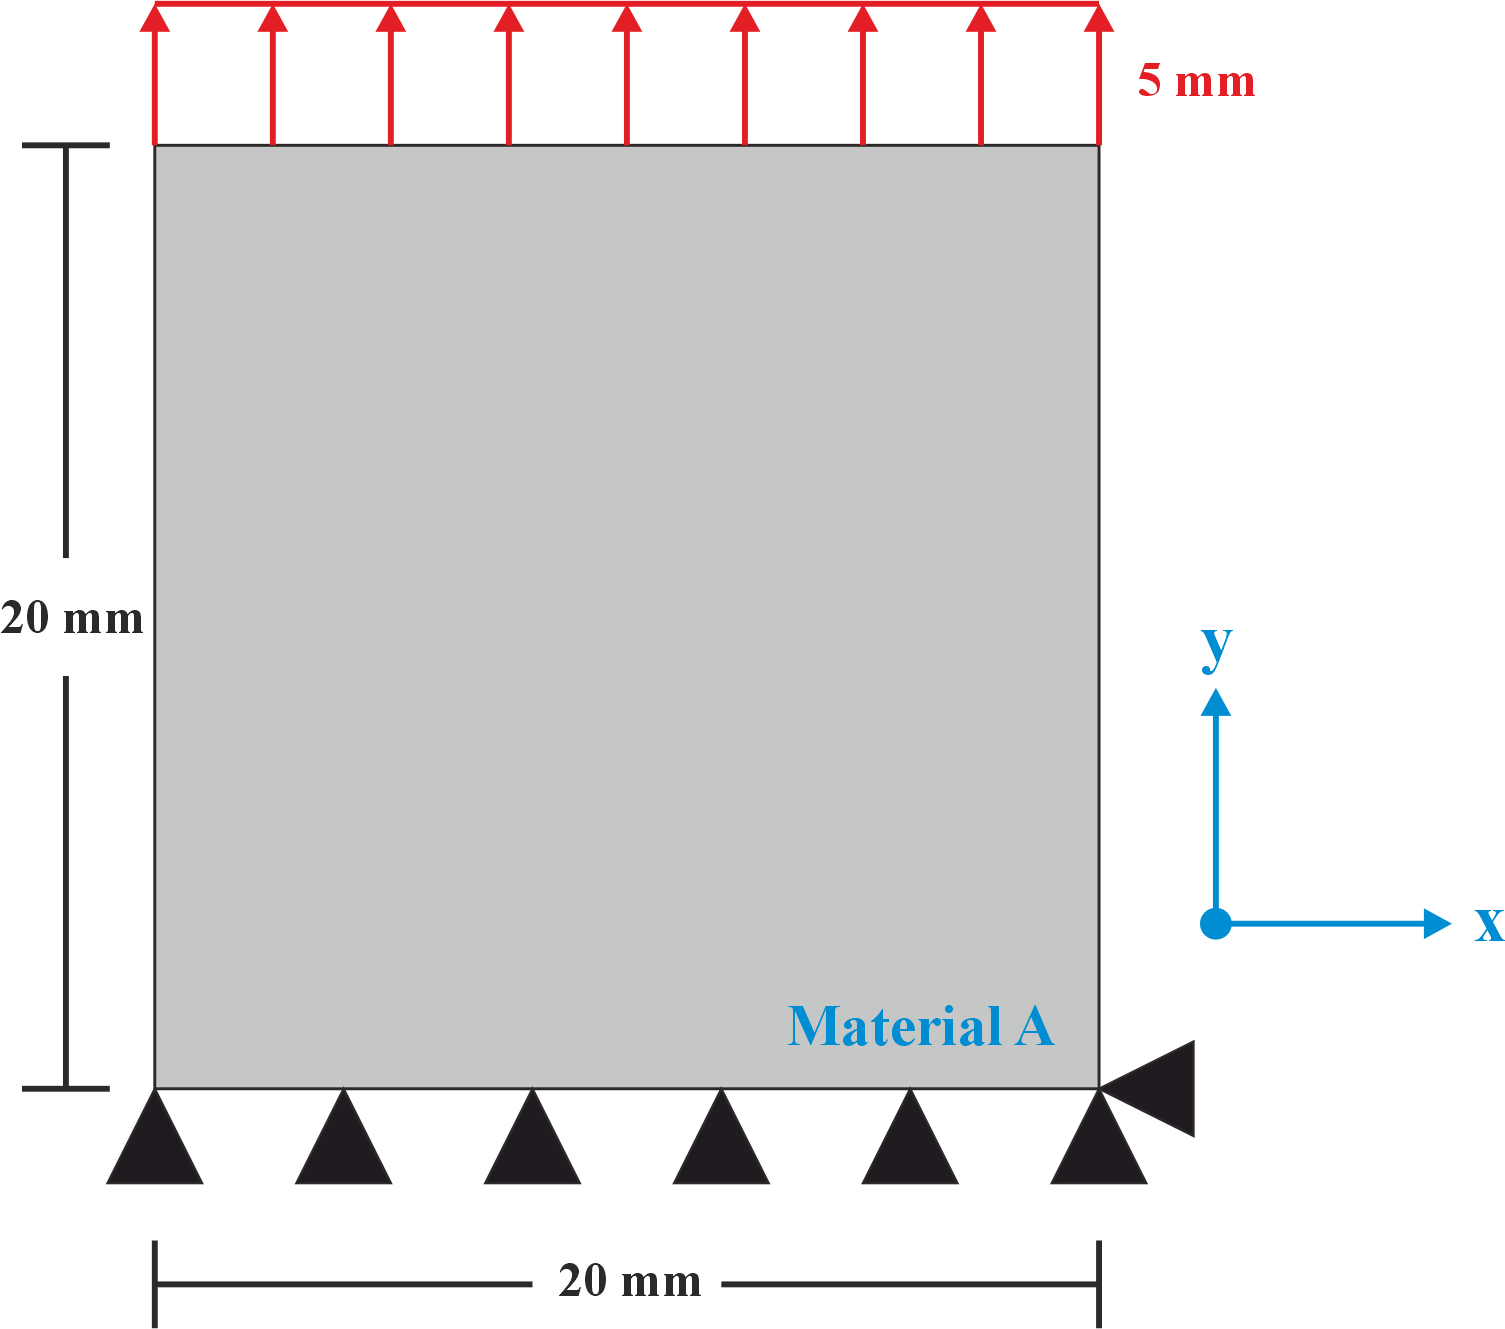
\includegraphics[width=0.5\textwidth]{images/TaskQ1.png}
        \caption{Baseline plate geometry with defined material A. Two boundary conditions are applied, which are the 
        fixed support restriction in y direction on the bottom line of the plate, fixed support point on the bottom right point restriction to 
        x direction, and constant distribution of displacement in y positive direction on the top line of the plate, which has value of 5 mm.}
        \label{fig:geometryQ1}
\end{figure}

    \item \textbf{Plate with Circular Inclusion:} Same as the baseline plate, but with a circular inclusion of radius $r=4$ mm located at the center or specified position.
\begin{figure}[H]
        \centering
            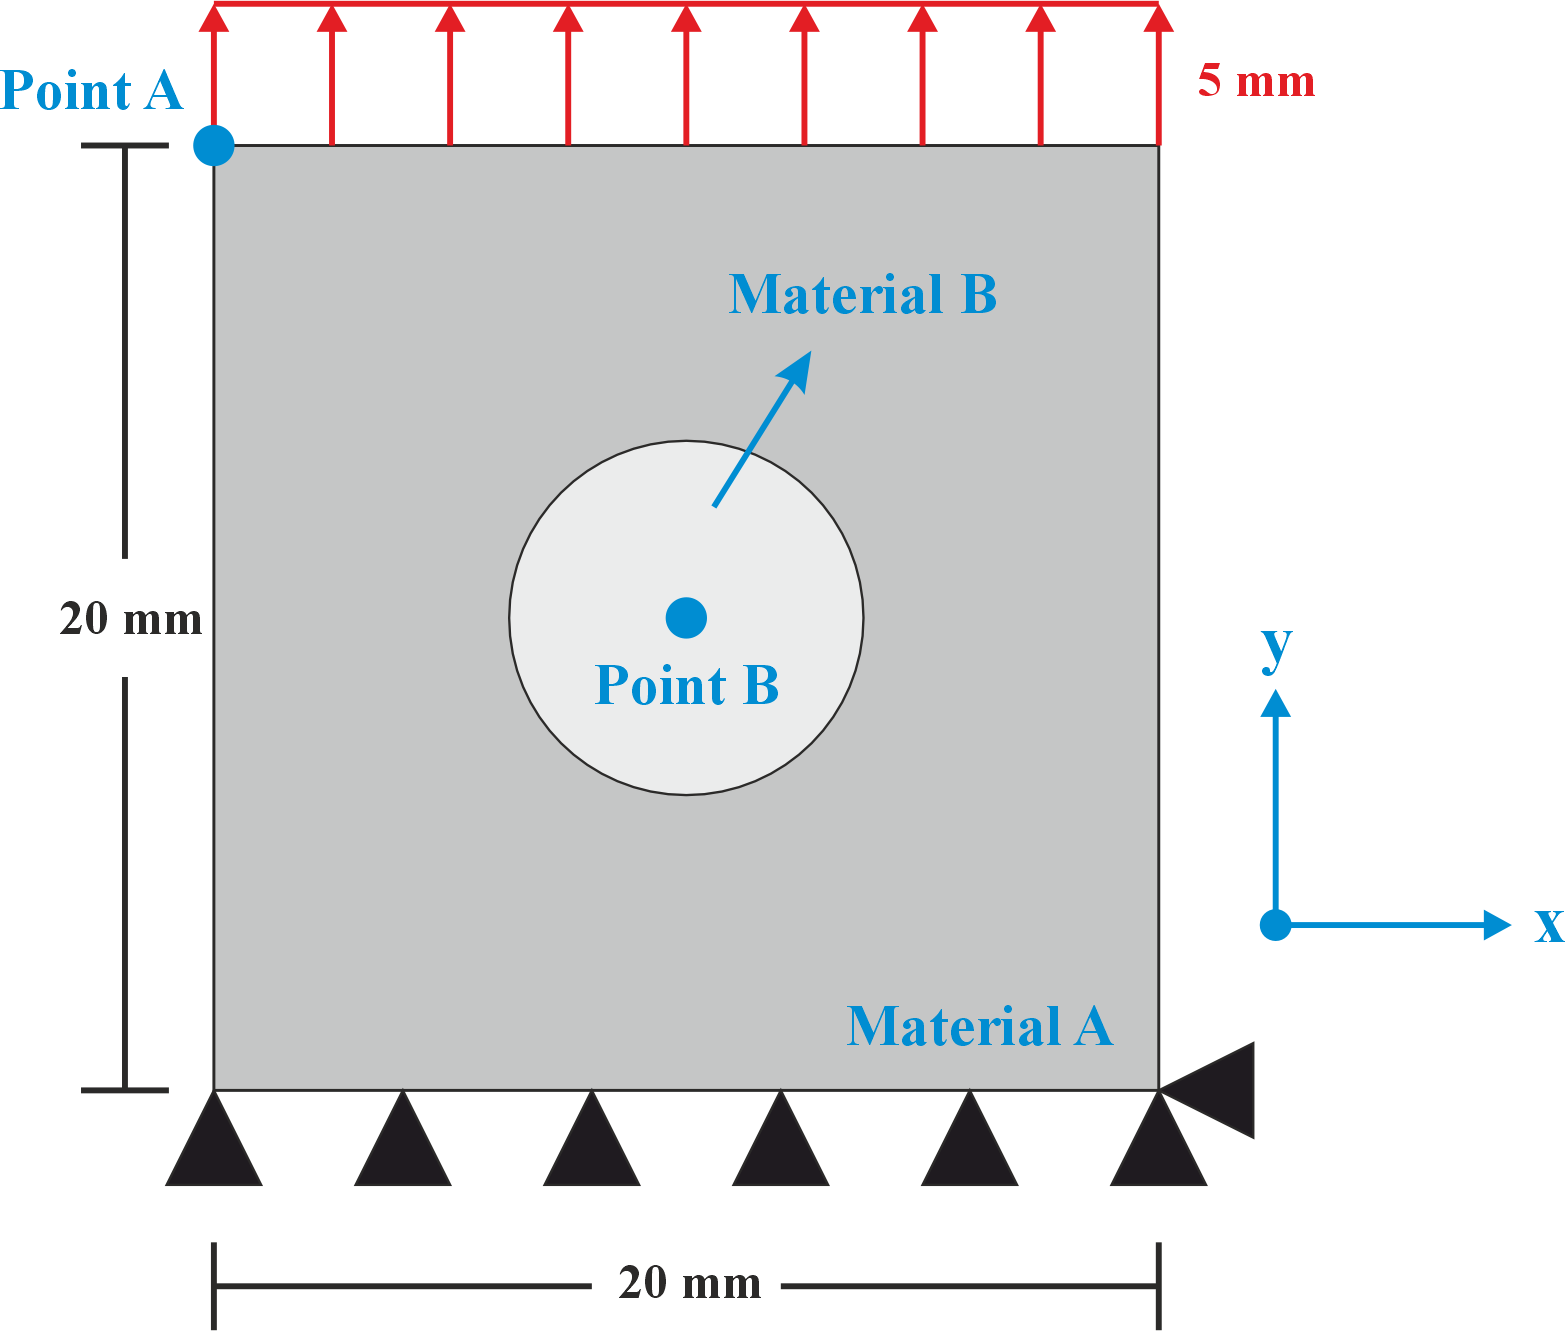
\includegraphics[width=0.5\textwidth]{images/TaskQ2.png}
        \caption{Plate with circular inclusion and defined material B. Boundary conditions are the same as in Task 1 shown in Figure~\ref{fig:geometryQ1}.}
        \label{fig:geometryQ2}
\end{figure}
\end{enumerate}
\subsection{Material Properties}
\hspace*{2em}The material properties used in the analysis are provided in the task definition. However, 
some parameters must be manually calculated based on the author's Immatrikulation Nummer in the very first section.
In Task 1, material A (see Table~\ref{tab:materialA-properties}) is applied and considered as an elastic-plastic isotropic material, 
characterized by Young's modulus $E$, Poisson's ratio $\nu$, yield stress $\sigma_{ya}$, ultimate tensile strength $\sigma_{f}$, 
and strain at fracture $\epsilon_{f}^{f}$.
For Task 2, which includes an additional central inclusion of material B, it is defined as an elastic-plastic material 
with anisotropic properties, meaning its characteristics vary in three orthogonal directions. 
In particular, the plastic behavior is described in Table~\ref{tab:materialB-plasticproperties},
where Hill's yield criterion is employed. Hill's coefficients $R_{ij}$ for $i,j = 1,2,3$ must be 
specified for each direction to calculate the corresponding Hill's parameters for stress and strain evaluation.


\begin{table}[H]
    \centering
    \caption{Elastic and plastic properties of material A.}
    \label{tab:materialA-properties}
    \begin{tabular}{lllll}
        \toprule
        E (GPa) & $\nu$ & $\sigma_{ya}$ (MPa) & $\sigma_{f}$ (MPa) & $\epsilon_{f}^{f}$ \\
        \midrule
        240 & 0.3 & 360 & 550 & 0.4 \\
        \bottomrule
    \end{tabular}
\end{table}

\begin{table}[H]
    \centering
    \caption{Elastic properties of material B.}
    \label{tab:materialB-elasticproperties}
    \begin{tabular}{lllllllll}
        \toprule
            \centering $E_1$ (GPa) & $E_2$ (GPa) & $E_3$ (GPa) & $\nu_{12}$ & $\nu_{13}$ & $\nu_{23}$ & $G_{12}$ (MPa) & 
            $G_{13}$ (MPa) & $G_{23}$ (MPa) \\
            \midrule
            \centering 210 & 220 & 230 & 0.3 & 0.31 & 0.32 & 80 & 84 & 87 \\
            \bottomrule
    \end{tabular}
\end{table}

\begin{table}[H]
    \centering
    \caption{Plastic properties of material B.}
    \label{tab:materialB-plasticproperties}
    \begin{tabular}{lllllllll}
        \toprule
            \centering $R_{11}$ & $R_{22}$ & $R_{33}$ & $R_{12}$ & $R_{13}$ & $R_{23}$ & $\sigma_{yb}$ & 
            $\sigma_{f}$ (MPa) & $\epsilon_{p}^{f}$  \\
            \midrule
            \centering 1 & 1.2 & 1.25 & 0.8 & 0.85 & 0.95 & 280 & 450 & 0.5 \\
            \bottomrule
    \end{tabular}
\end{table}
\subsection{Meshing}
\hspace{2em}The models for this tasked are differs into two different 
meshes types, which first one is the homogeneous baseline plate 
with a uniform mesh size distribution, and the 
second one is the plate with circular inclusion,
which it has a customized mesh distribution in order to 
take account creating symmetrical meshes distribution 
across the geometry variant. Creating meshes for geometry with inclusion
should be taking care of some aspects, for instance, defining the distribution 
pattern of the mesh size, which the program mesh algorithm from Abaqus
CAE can automatically generate a symmetrical mesh distribution. Hence, 
defining geometry partition is having an important role in order to achieve
a good mesh distribution. Another important note, that it is crucial
to assign as a quad-structured mesh in the mesh control setting in order to enhance the symmetrical property of the mesh 
instead of auto generating the mesh, which will create a high-probable randomized mesh distribution. The following figures show the meshing
for both models. Noted that in this assignment, we will not use the
reduced integration element, which in the end the logarithmic strain
will be shown instead of the regular strain. 
\begin{figure}[H]
    \centering
    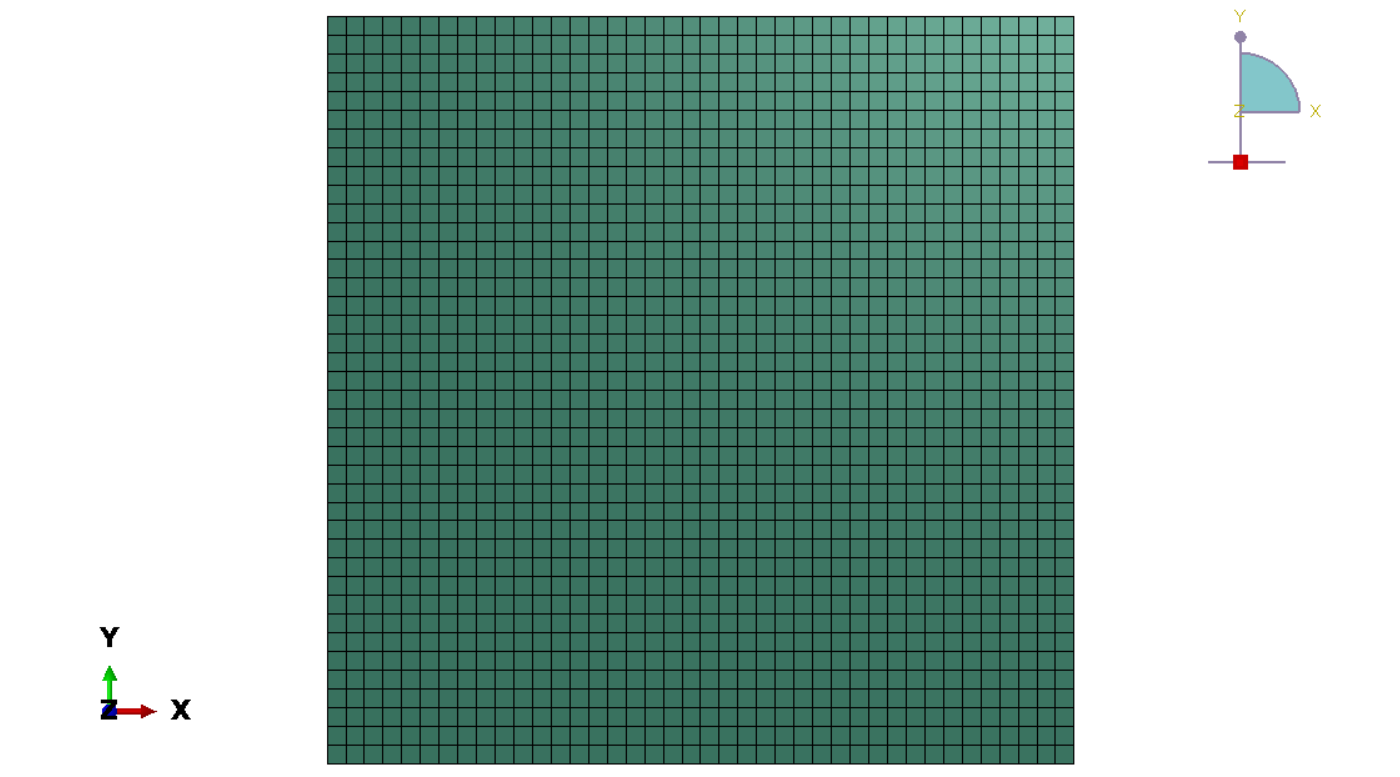
\includegraphics[width=1\textwidth]{images/MeshQ1.png}
    \caption{Mesh for the baseline plate with uniform mesh size distribution, 
    with total of 1600 elements. The mesh size is defined as 0.25 mm
    gap size with set up for both plane stress and plane strain
    conditions. CPS4, which is a 4-node bilinear plane stress/strain quadrilateral, is applied for task 1 mesh configuration}
    \label{fig:MeshQ1}
\end{figure}

\begin{figure}[H]
    \centering
    \begin{minipage}{0.48\textwidth}
        \centering
        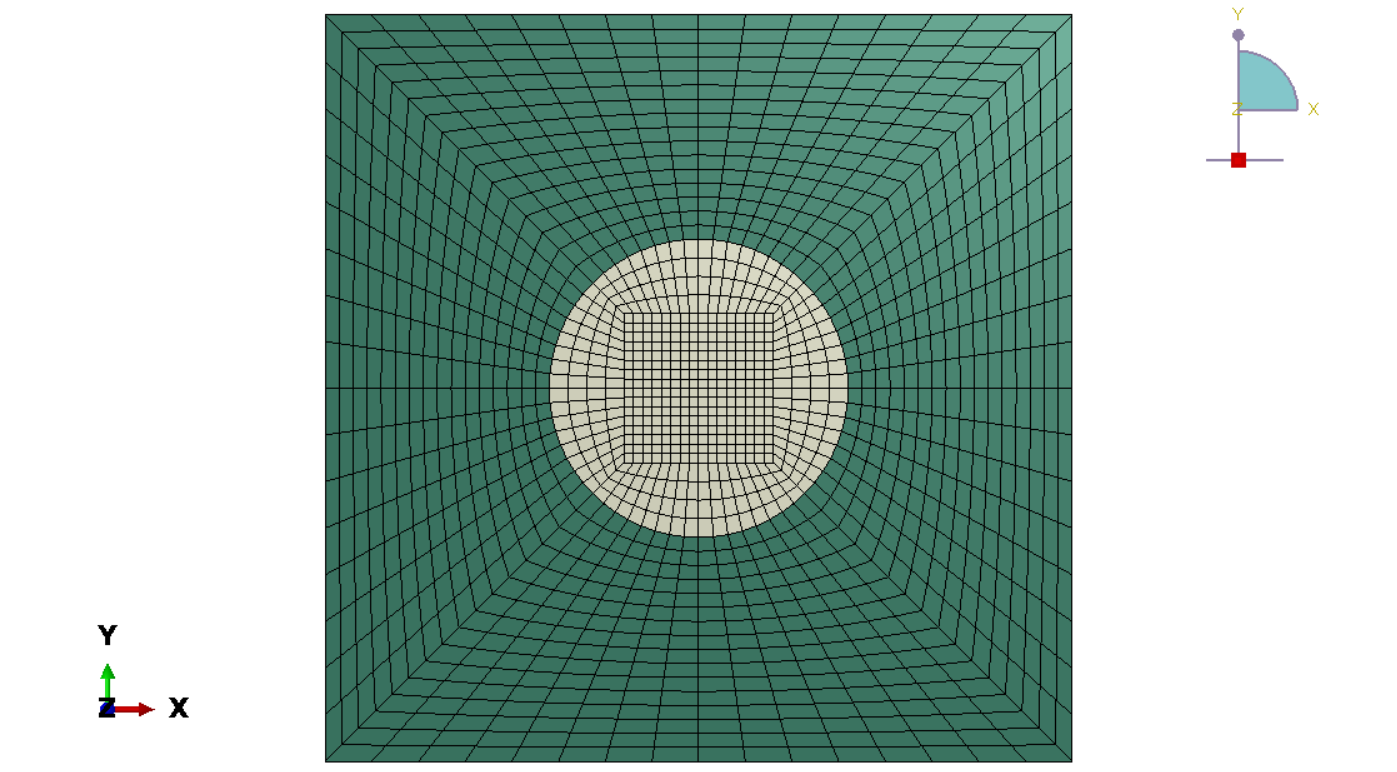
\includegraphics[width=\textwidth]{images/MeshQ2.1.png}
        \caption{Mesh for the plate with circular inclusion for the coarse variation
        with 1536 elements. CPS4, which is a 4-node bilinear plane stress quadrilateral, is applied for task 2 coarse mesh configuration}
        \label{fig:MeshQ2.1}
    \end{minipage}\hfill
    \begin{minipage}{0.48\textwidth}
        \centering
        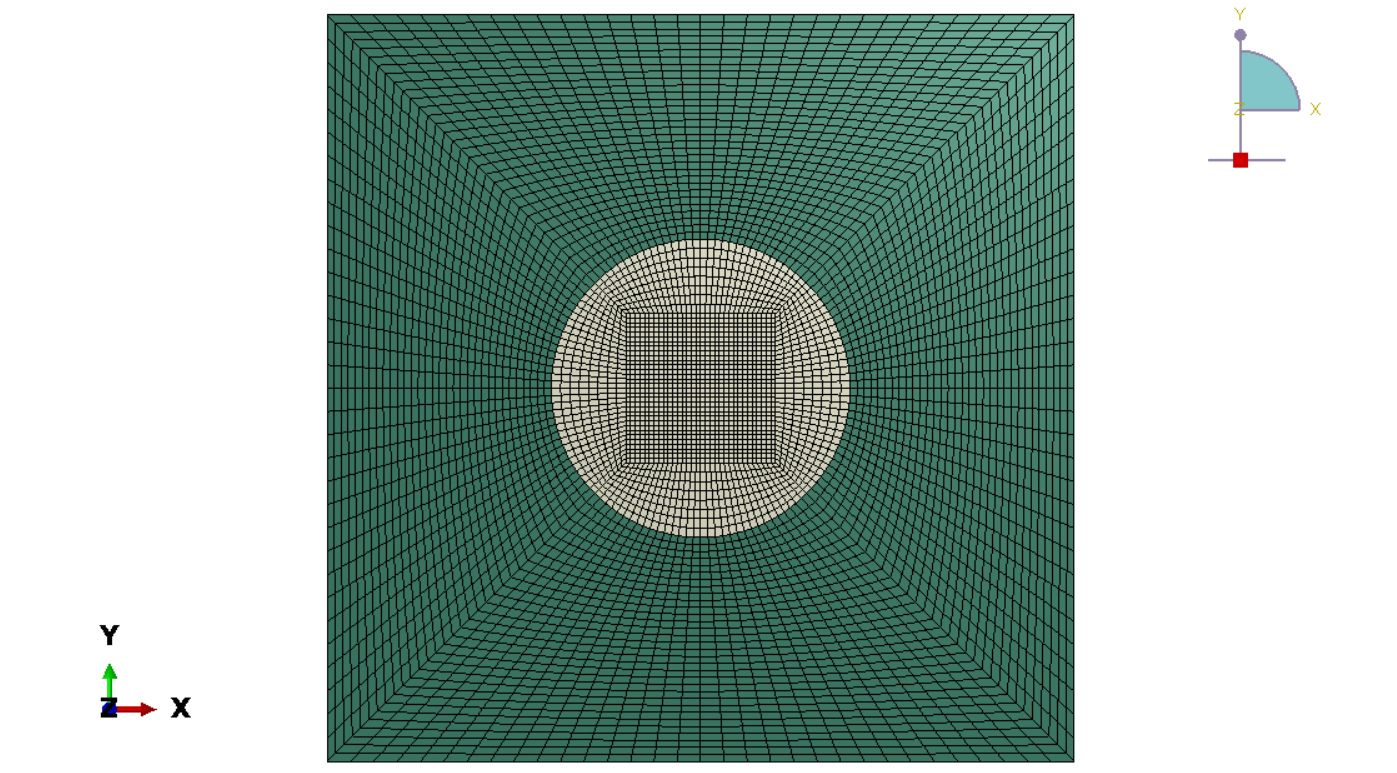
\includegraphics[width=\textwidth]{images/MeshQ2.2.png}
        \caption{Mesh for the plate with circular inclusion for fine mesh variation
        with 6144 elements. CPS4, which is a 4-node bilinear plane stress quadrilateral, is applied for task 2 fine mesh configuration}
        \label{fig:MeshQ2.2}
    \end{minipage}
\end{figure}
\section*{Results and Discussion}

\subsection*{Q1: Mechanical Response Analysis for Baseline Plate}

\textit{$\dots$ Plot the global stress-strain curve from the numerical model using two different methods: (1)
by extracting local stress and strain values from average over all the elements at the top edge,
and (2) by computing stress and strain from the total reaction force and total displacement at
the top edge nodes. Compare and discuss the stress-strain curves obtained from both methods.
Then, select the curve from the second method and clearly mark and distinguish the elastic
region, the yield transition, and the strain hardening stage.}

\begin{figure}[H]
    \centering
    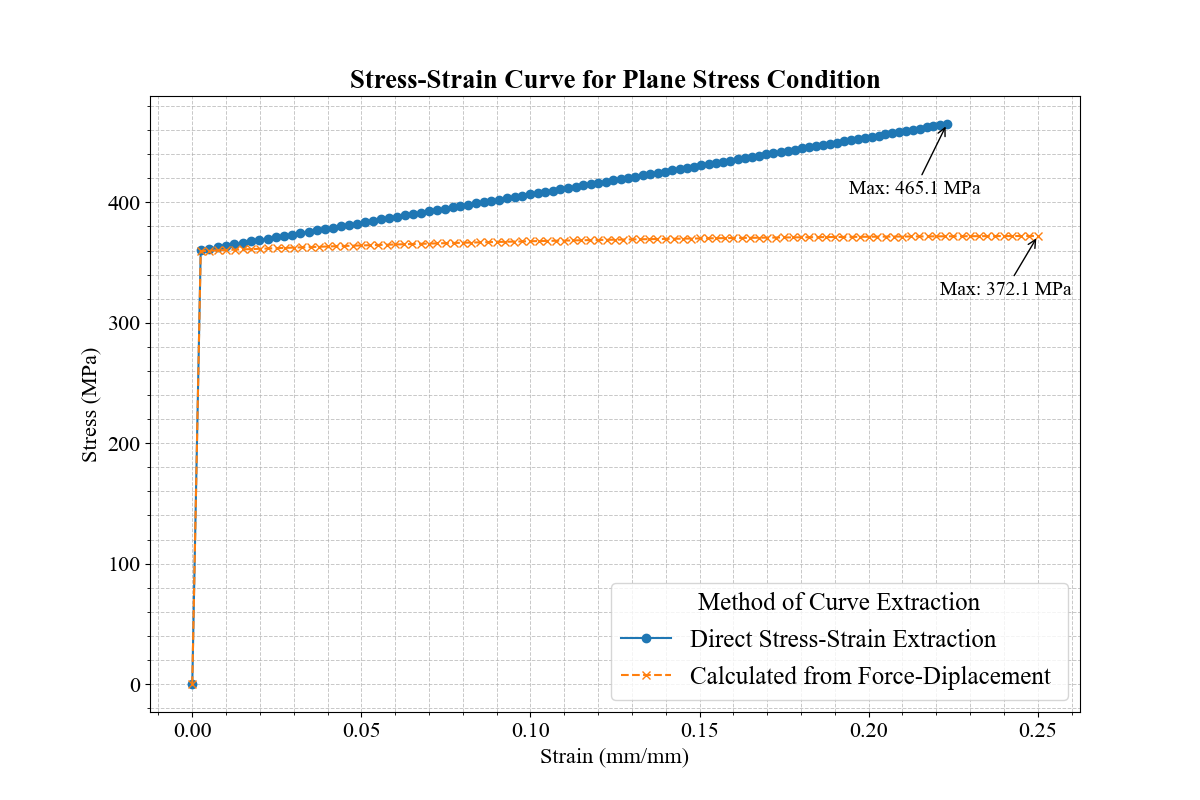
\includegraphics[width=1\textwidth]{visualize_tensileGraph/res/comparison_direct_calculated.png}
    \caption{Comparison of the stress-strain curves obtained from the force-displacement method and the direct stress-strain calculation 
    for the plane stress condition. The direct stress-strain curve is obtained by extracting the stress $\sigma_{22}$ 
    and strain $\varepsilon_{22}$ directly from the history output, which includes all nodes along the top edges of the baseplate. 
    The calculated force-displacement data is obtained by extracting the force $F_{22}$ and displacement $U_{22}$ from the 
    history output, which also includes all nodes along the top edges of the baseplate.
Then, the stress is obtained by dividing the force by the surface area normal to the loading direction, which is
$A=20 \; \text{mm}^2$. The strain is calculated by taking the displacement and dividing it by the baseplate's original length, which is 
$L=20 \; \text{mm}$, in the direction of loading.} 
    \label{fig:ComparisonDirectCalculated}  
\end{figure}

\hspace{2em}Based on Figure~\ref{fig:ComparisonDirectCalculated}, both stress-strain curves obtained from the two 
methods show different behavior. In the plastic flow region or often called as strain hardening stage, 
the direct method produces a significant slope, while the calculated method shows a constant slope almost most likely 0 gradient, 
indicating the material behaves as perfectly plastic without hardening. 
This difference occurs because, in the direct stress-strain extraction method, the solver calculates the true stress-strain 
by taking account geometric changes such as the cross-sectional area reduction. In the plastic flow
region, the geometry undergoes necking, which decreases the cross-sectional area and leads to higher 
stress values. This extracted value is often called the true stress-strain diagram, as it uses the logarithmic 
strain and accounts for the reduction in cross-sectional area. Therefore, using this method will enable us to see the hardening
region during the plastic flow process.

\hspace{2em}In the calculated from force-displacement method, the stress obtained by calculating the total force produced in the top nodal line of the baseplate divided by a constant area value, which here
the stresses are most likely does not increase in the plastic region, since it use the original cross-sectional area as the dominator. This method also applied to calculate the strain, which only
divide the displacement with the original length of the baseplate. This method is often used to create the engineering stress-strain curve. In the experimental tensile test, 
this method is often used to obtain the stress-strain curve, 
since the obtained test data is only force and displacement of the extensometer. 

\hspace{2em}To distinguish the critical event point, on figure~\ref{fig:distinguishImportantRegion} is the detailed description of the critical
events during the loading of the axial load in the top side of the plate. 

\begin{figure}[H]
    \centering
    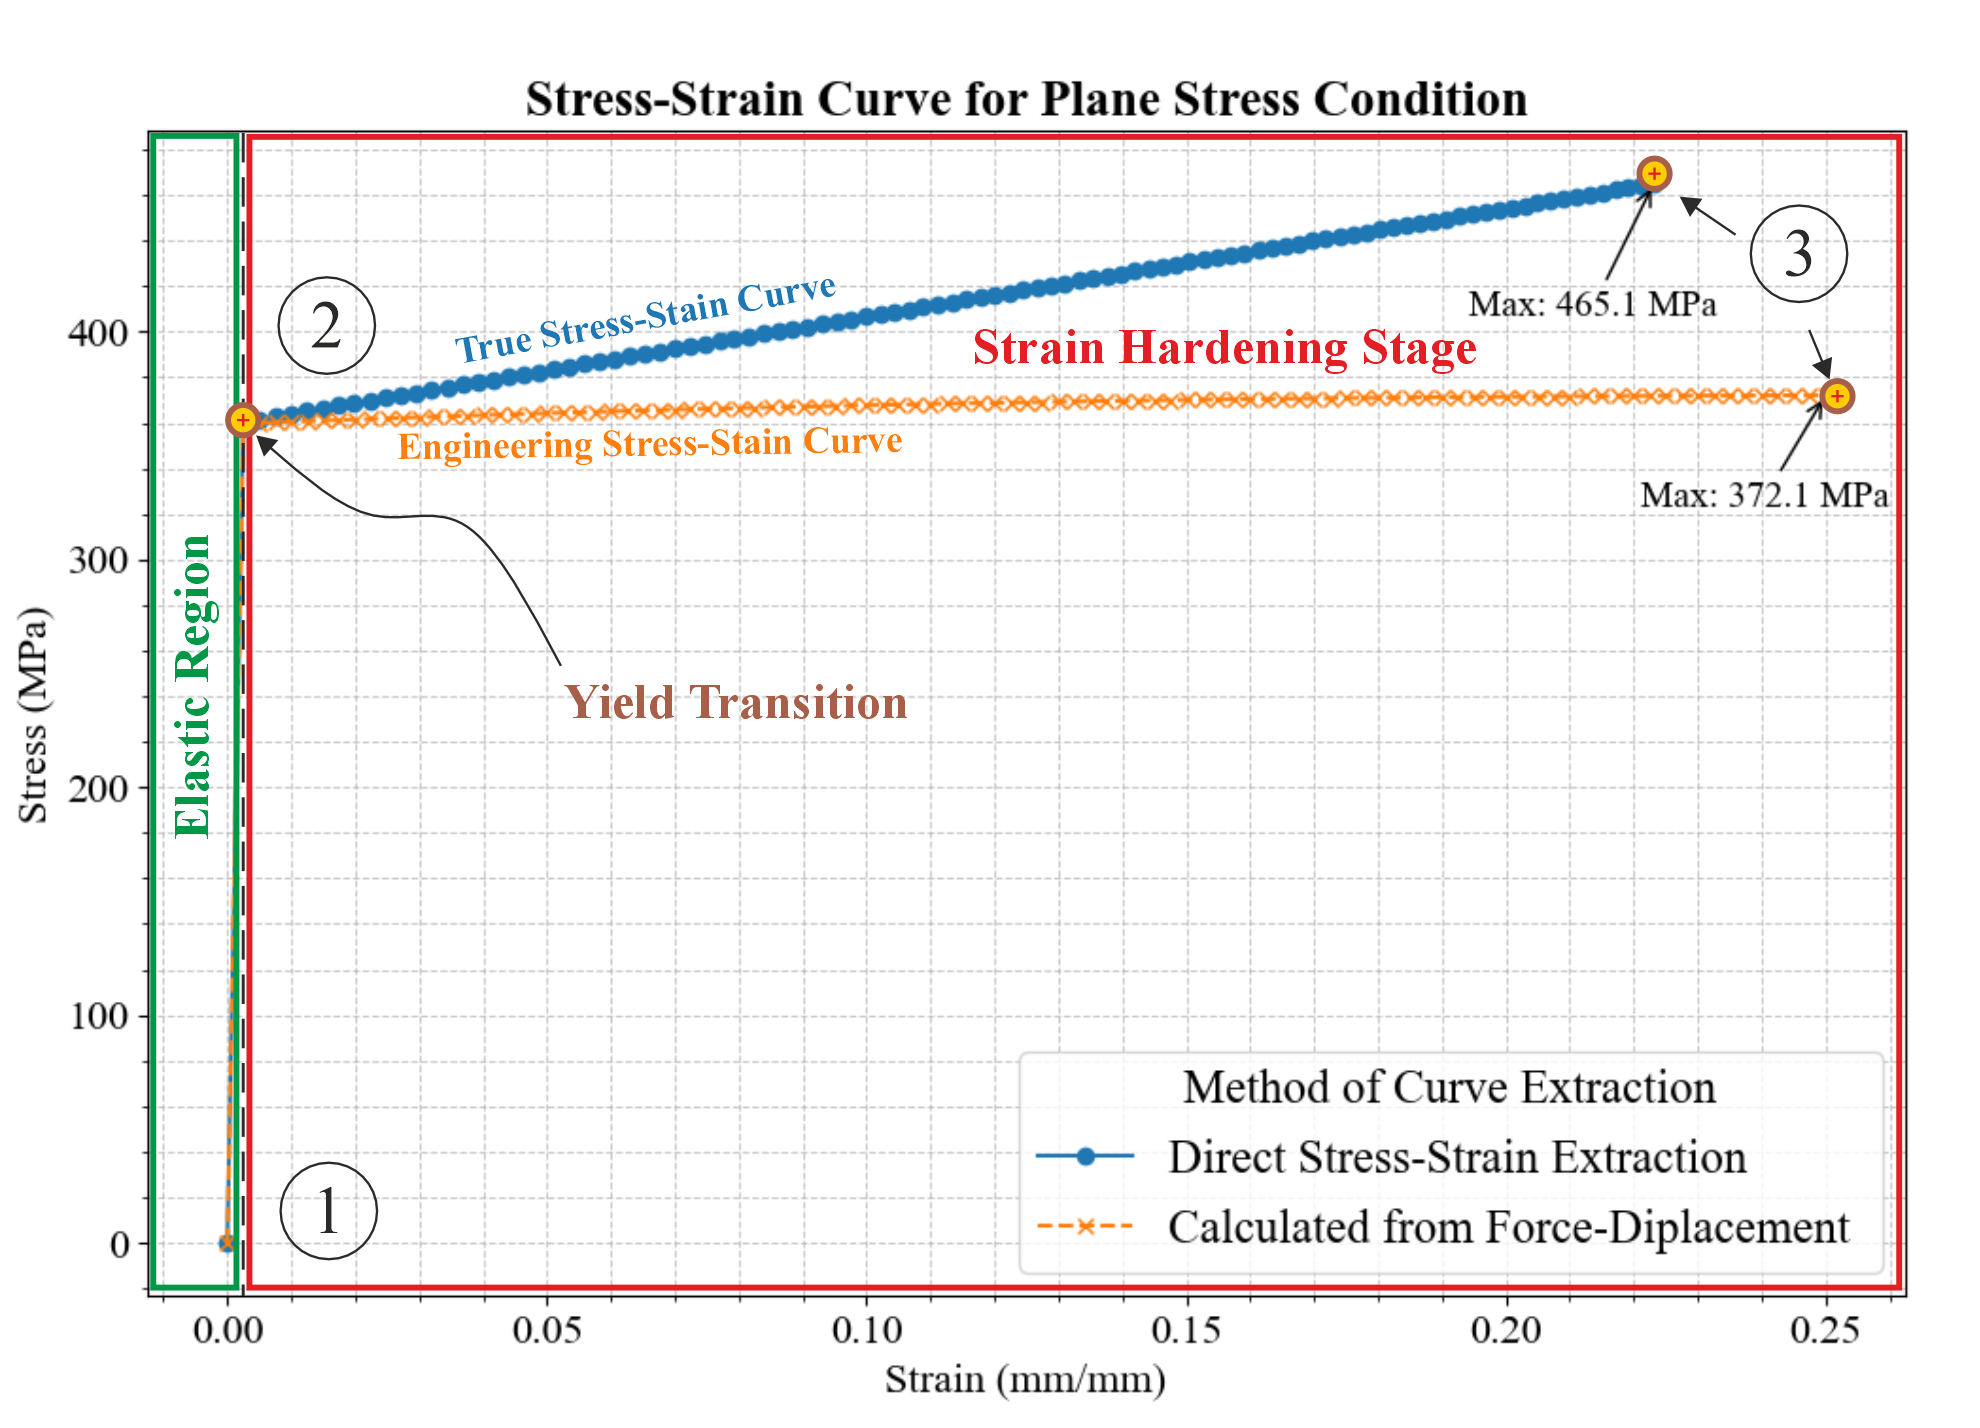
\includegraphics[width=0.85\textwidth]{visualize_tensileGraph/res/comparison_direct_calculated_modified.png}
    \caption{Annotation of the elastic region, yield stress transition, and the strain hardening stage figure. From point 1-2 is the elastic region, whereas 
    at point 2 it starts to yield transitioning to become plastic state. From point 2-3 is the strain hardening stage, as the material continuously plastically
    deformed until its fracture in point 3.}
    \label{fig:distinguishImportantRegion}
\end{figure}


\vspace{1em}
\textit{$\dots$ Set up the same model under plane strain conditions. Plot the stress-strain curve obtained from
method 2 for the new model.}

\begin{figure}[H]
    \centering
    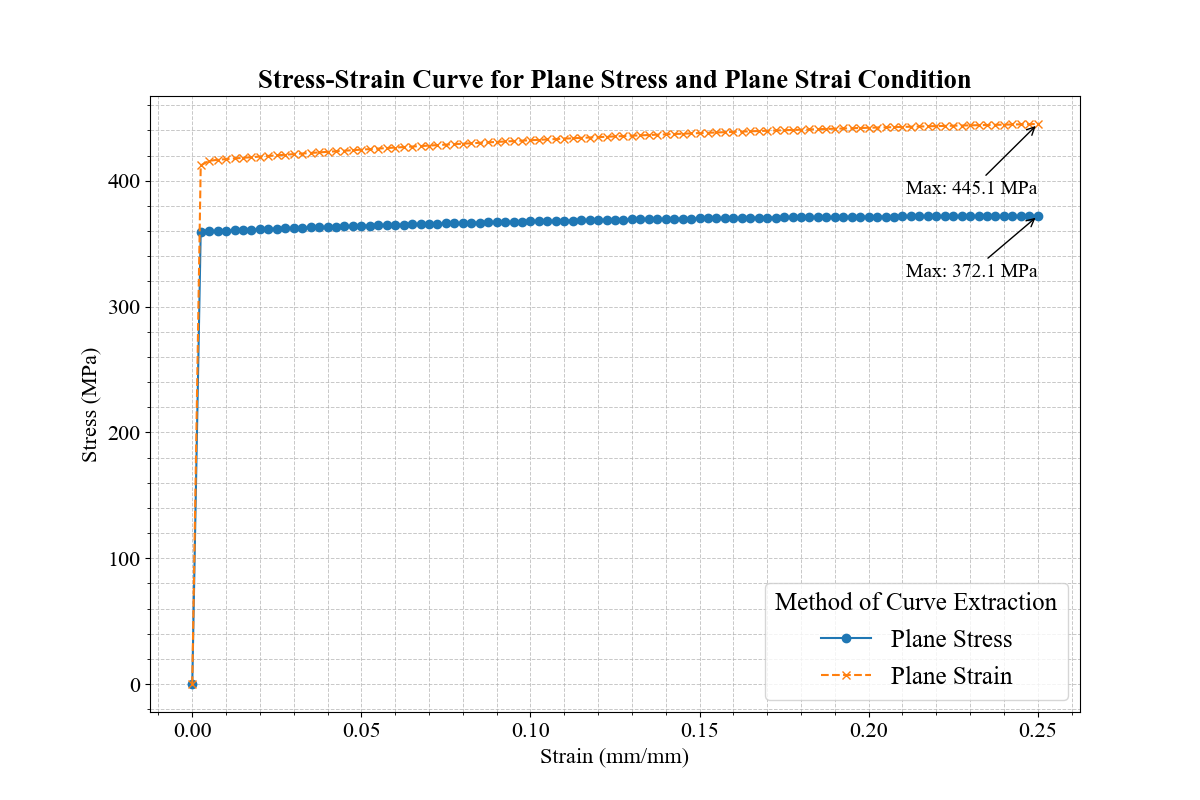
\includegraphics[width=1\textwidth]{visualize_tensileGraph/res/comparison_planeStress_planeStrain.png}
    \caption{Comparison of plane stress and plane strain conditions
    for the baseline plate with material A. The setting for plane stress and strain are distinguised by changing the type of meshing in
    Abaqus based on the condition.} 
    \label{fig:ComparisonDirectCalculated}  
\end{figure}

\textit{$\dots$ Compare and discuss the implications of choosing plane stress or plane strain conditions on
the mechanical behavior of the model.}
\vspace{1em}

\hspace{2em}Based on Figure~\ref{fig:ComparisonDirectCalculated}, the stress-strain curves for both plane stress and plane strain 
conditions show similar behavior in terms of producing young modulus, as well as the fracture stress.
Whereas the plane strain condition exhibiting a slightly higher yield stress.
This is expected, as the plane strain condition restricts deformation in the thickness direction, 
leading to higher stress values. This stress produced from the strain restriction in the thickness direction,
which will lead to produce additional stress component that will increase the overall stress generation. Therefore, choosing the 
plane stress condition is more appropriate for thin-plates analysis since it neglects the stress generated 
in the thickness direction. For plane strain condition, it is more suitable in a thick cross-section analysis. 

\newpage
\subsection*{Q2: Mechanical Response Analysis for Plate with Circular Inclusion}

\textit{$\dots$Plot the global stress-strain curve of the model with inclusion, by computing it from the total
reaction force and the total displacement of top edge nodes (method 2).}
\vspace{1em}

In this section, we analyze the mechanical response of the plate with a circular inclusion and compare it to that of the homogeneous baseline plate.

\begin{figure}[H]
    \centering
    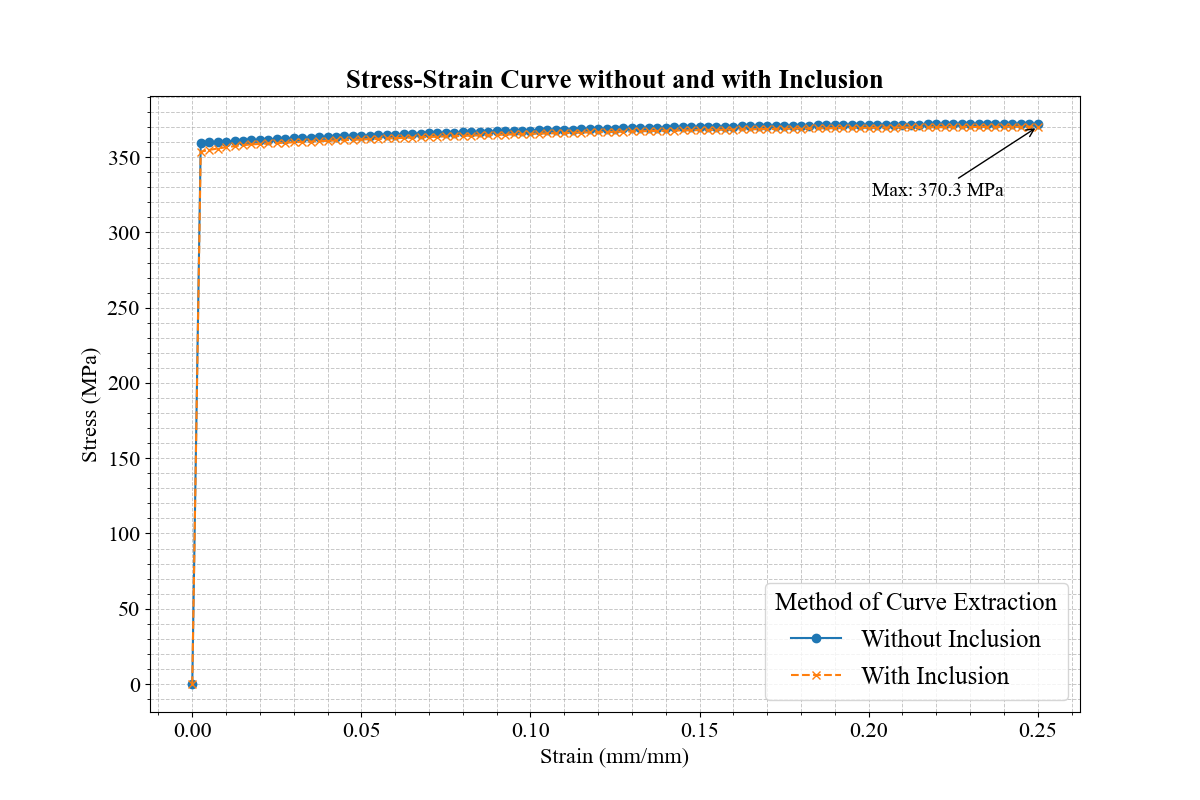
\includegraphics[width=1\textwidth]{visualize_tensileGraph/res/comparison_inclusion_non.png}
    \caption{Comparison of the stress-strain curves for the homogeneous baseplate and plate with circular
    inclusion. Plate with inclusion produced yield and fracture stress of $353.805 \; \text{MPa}$ and $370.276\; \text{MPa}$,
    while plate with inclusion has $359.574\; \text{MPa}$ and $372.058\; \text{MPa}$, respectively.}
    \label{fig:ComparisonInclusion}
\end{figure}


\textit{$\dots$Compare and discuss the stress-strain curve with Q1, with a focus on how their constitutive
models influence the transition from elastic to plastic behavior and explain how the added
inclusion affects the stress-strain curve.}
\vspace{1em}


\hspace{2em}From the response of the stress-strain curves for each plate cases, we can observe that the plate with inclusion
has slightly lower yield stress compared to the homogeneous plate. This not only shift the yield point, but also reduce the ultimate tensile 
stress and the end of the stress, which also has slightly smaller value compare to the plate without inclusion. If we take a look at the
constitutive model based on table ~\ref{tab:materialA-properties}, ~\ref{tab:materialB-elasticproperties}, and ~\ref{tab:materialB-plasticproperties},
both material shows different properties, which material B tends to be a "softer" material compare to A. This can be seen from the yield $\sigma_{y}$ 
and fracture $\sigma_{f}$ stresses, whereas material B has the lower value in comparison to material A. 

\hspace{2em}Another reason, which may potentially come up, why material B is softer than material A is because it's also taking account to the anisotropic behavior, while
in contrast material A has the isotropic property. Hence, the properties of material B is dependent for every load direction. This can be described
by the defined anisotropic yield stress ratio $R_{ij}$, where it tells us the ratio of yield stress for every axis with respect to the based yield
stress. Hence, these non-homogeneous properties may be the game changer role in decreasing the material properties with respect to 
single loading case. However for this case, the main aspect that weakens the material B properties is dominated by the yield and fracture stress reduction,
where the difference is quite prominent. Therefore, anisotropic property in this case does not play the main role in decreasing the strength of material B. 

\hspace{2em}Since the inclusion size is not dominating the whole area of the plate, it actually played quite small significant role in softening
the overall plate properties. This can be proof by observing the elastic region, whereas the elastic modulus or the slope of the curve in this 
region are still non-distinguishable, meaning that material A is still dominating the properties. In the atomistic level, it can be 
explained that material A still able to hold the whole material plate in the elastic region. However at some point, the material cannot
withstand the load in the elastic region since the "number of material A in plate with inclusion is less than the material A in plate without inclusion", 
then it starts to yield faster. Thus, it can be concluded that since the inclusion size ratio is not significantly larger than the non-inclusion material,
it affects slightly weakening the overall stress, causing the plate with inclusion to yield and fracture in slightly lower stress value.   



\newpage
\subsection*{Q3: Local Stress Field Distribution and Analysis}
\textit{$\dots$Create a contour plot of the key stress components (S11, S22, S12, MISES) at the final time
step and discuss the results for different regions.}
\vspace{1em}

Hence, we will analyze the stress distribution for baseplate with inclusion. 
\vspace{1em}

\begin{figure}[H]
    \centering
    \begin{minipage}{0.48\textwidth}
        \centering
        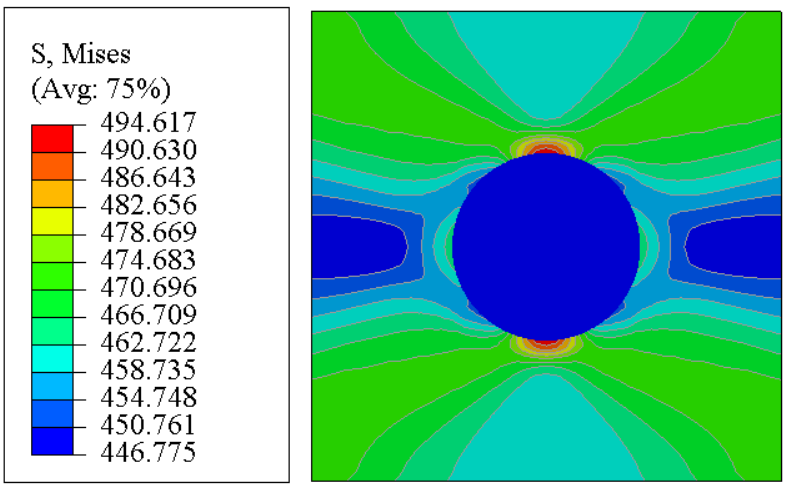
\includegraphics[width=\textwidth]{images/MISES.png}
        \caption*{(a) $\sigma_{vM}$}
    \end{minipage}
    \hfill
    \begin{minipage}{0.48\textwidth}
        \centering
        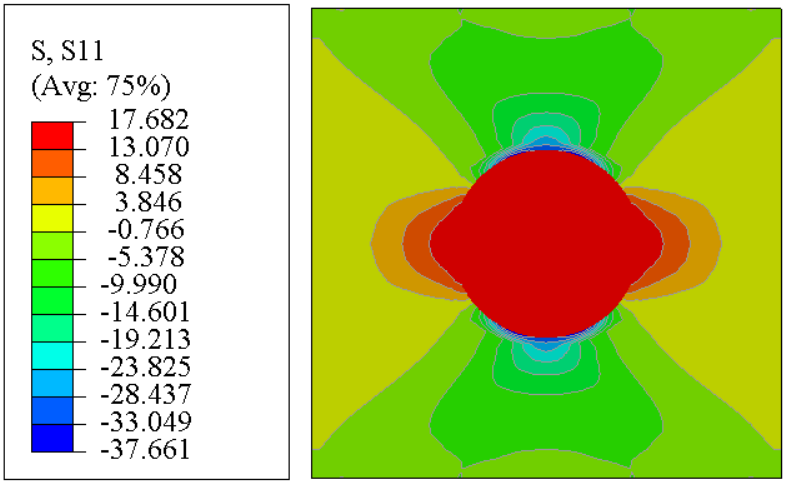
\includegraphics[width=\textwidth]{images/S11.png}
        \caption*{(b) $S_{11}$}
    \end{minipage}
    \vspace{1em}
    \begin{minipage}{0.48\textwidth}
        \centering
        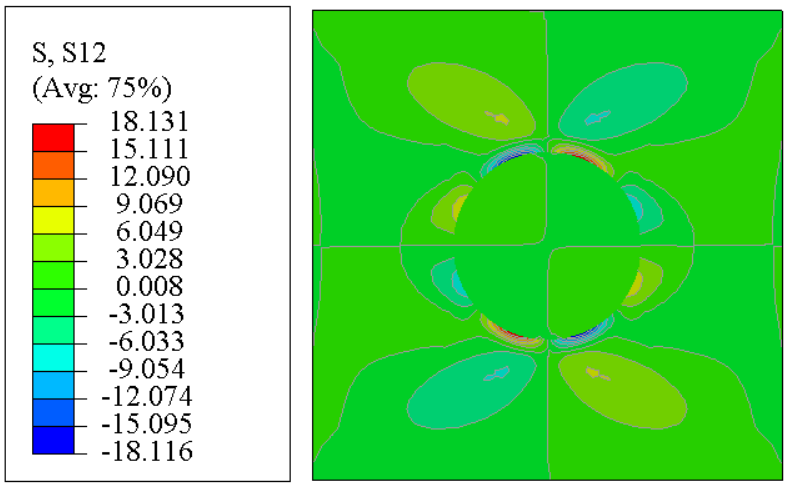
\includegraphics[width=\textwidth]{images/S12.png}
        \caption*{(c) $S_{12}$}
    \end{minipage}
    \hfill
    \begin{minipage}{0.48\textwidth}
        \centering
        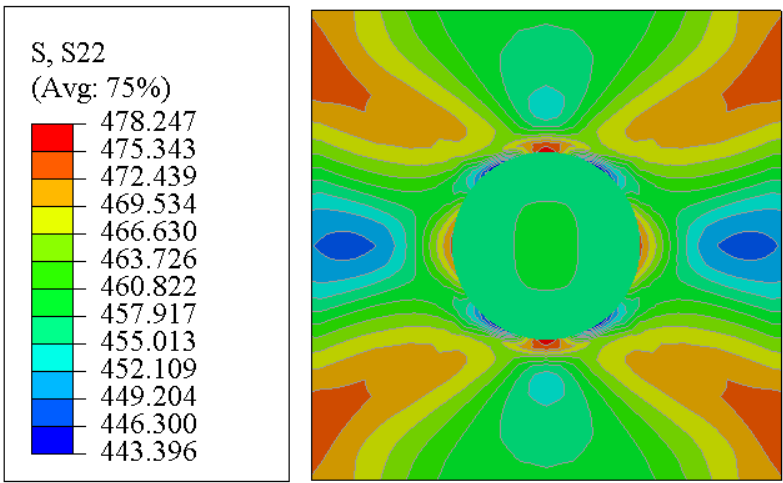
\includegraphics[width=\textwidth]{images/S22.png}
        \caption*{(d) $S_{22}$}
    \end{minipage}
    \caption{Contour plots of (a) von Mises stress, (b) $S_{11}$, (c) $S_{12}$, and (d) $S_{22}$ for the plate with circular inclusion.
    Noted that all the used unit for this plot is MPa for stress unit.}
    \label{fig:stressFieldsall}
\end{figure}

\hspace{2em}From the stress distribution contour plots in Figure~\ref{fig:stressFieldsall},
we can see some several characteristics of the stress behavior in the plate with circular inclusion.
\begin{itemize}
    \item For the von Mises stress distribution in part (a), it shows a discontinuous stress distribution between the inclusion 
    and the outer non-inclusion part. This is because both material A (in the non-inclusion area) and material B have different 
    material properties, where material B tends to be softer compared to material A. This implies that material B will deform more 
    easily, requiring lower stress compared to material A. Two high stress concentrations are observed at the top and bottom circular 
    circumferences outside the inclusion, indicating the locations of the highest and most critical stress.
    \item As in the $S_{11}$ distribution, the stress tends to have negative values in the non-inclusion area. 
    This is because, as the plate deforms, the geometry is compressed toward the right side, parallel to the x-axis. Hence, 
    it produces a reaction force opposite to the movement, resulting in negative stress values, which indicate that the material 
    is being compressed in the x direction. However, a different case is observed in the inclusion part, where the stress is 
    dominated by tensile stress rather than compressive, as shown by the positive values throughout the inclusion area.
    \item In the $S_{12}$ plot, the shear stress value tends to be small in the whole part of the plate. However, there
    are some shear stress generated in the boundary between the inclusion and the homogeneous part of the
    plate, which here causes by the friction force generated by the movement of materials. 
    \item For the stress plot in the y-direction $S_{22}$, the highest stress is mostly generated at the four edges of material A 
    and at the interface between material A and inclusion material B. 
    This is also caused by the discontinuity in material properties between A and B. 
    Another observation is that the stress in the y-direction has the highest value compared to the other stress components, 
    since the loading direction is parallel to this axis.
\end{itemize}

\newpage
\subsection*{Q4: Comparison Analysis at Point A}
\textit{$\dots$Calculate the von Mises equivalent stress and equivalent plastic strain at point A in Figure 2
based on the analytical equations given in the lecture and the stress and plastic strain
components obtained from the simulation. Compare the results to the values of MISES and
PEEQ from the Abaqus postprocessing menu.}
\vspace{1em}

To calculate the von Misses equivalent stress and equivalent plastic strain at point A analytically, 
we can use following equations:
\begin{equation}
    \sigma_{eq, hill} = \sqrt{
        F(\sigma_{22}-\sigma_{33})^2 + 
        G(\sigma_{33}-\sigma_{11})^2 + 
        H(\sigma_{11}-\sigma_{22})^2 + 
        2L\sigma_{23}^2 + 
        2M\sigma_{31}^2 + 
        2N\sigma_{12}^2
    }
    \label{eq:hill_yield}
\end{equation}

\begin{equation}
    \varepsilon_{eq} = \sqrt{\frac{F\varepsilon_{pl,11}^2 + G\varepsilon_{pl,22}^2 + H\varepsilon_{pl,33}^2}{FG+FH+GH} + \frac{2\varepsilon_{pl,12}^2}{N}}
    \label{eq:equivalent_plastic_strain}
\end{equation}

where $\varepsilon_{pl,33}=-(\varepsilon_{pl,11}+\varepsilon_{pl,22})$. Hence all of the constant in the equations
are described using $R_{ij}$, where these variable describe the ratio of plasticity between the preceeding directions and the based
yield stress:

\begin{align*}
F &= \frac{1}{2} \left[ \frac{1}{(R_{22})^2} + \frac{1}{(R_{33})^2} - \frac{1}{(R_{11})^2} \right] \\
G &= \frac{1}{2} \left[ \frac{1}{(R_{33})^2} + \frac{1}{(R_{11})^2} - \frac{1}{(R_{22})^2} \right] \\
H &= \frac{1}{2} \left[ \frac{1}{(R_{11})^2} + \frac{1}{(R_{22})^2} - \frac{1}{(R_{33})^2} \right] \\
L &= \frac{3}{2(R_{23})^2} \\
M &= \frac{3}{2(R_{31})^2} \\
N &= \frac{3}{2(R_{12})^2}
\end{align*}

At point A, since it use material A and it is an isotropic material, 
therefore we can assume all of the $R_{ij}$ are equal to 1. Therefore, the hill's
equivalent stress and strain can be simplified as follows:
\begin{equation}
    \sigma_{eq, hill} = \sqrt{\frac{1}{2}((\sigma_{22}-\sigma_{33})^2 + (\sigma_{33}-\sigma_{11})^2 + (\sigma_{11}-\sigma_{22})^2 + 6\sigma_{23}^2 + 6\sigma_{31}^2 + 6\sigma_{12}^2)}
\end{equation}
\begin{equation}
    \varepsilon_{eq} = \sqrt{\frac{2(\varepsilon_{pl,11}^2 + \varepsilon_{pl,22}^2 + (\varepsilon_{pl,11}+\varepsilon_{pl,22})^2)}{3} + \frac{4\varepsilon_{pl,12}^2}{3}}
\end{equation}

At point A, the value of the stress and strain can be extracted directly from Abaqus. Following is the tabulized result for each 
variable that are needed for the calculation.
\begin{table}[H]
    \centering
    \caption{Extracted stress and strain components at point A from Abaqus.}
    \label{tab:pointA-results}
    \begin{tabular}{llllll}
        \toprule
        $\sigma_{11}$ (MPa) & $\sigma_{22}$ (MPa) & $\sigma_{12}$ (MPa) & $\varepsilon_{pl,11}$ & $\varepsilon_{pl,22}$ & $\varepsilon_{pl,12}$\\
        \midrule
        -2.61 & 472.16 & 1.24 & -0.1196 & 0.2388 & -0.0014\\
        \bottomrule
    \end{tabular}
\end{table}

Then we can use these data to calculate the equivalent von Mises stress and plastic strain. 

\begin{equation}
    \sigma_{eq, hill}^A = \sqrt{\frac{1}{2}((\sigma_{22}-0)^2 + (0-\sigma_{11})^2 + (\sigma_{11}-\sigma_{22})^2 + 6\sigma_{12}^2)} 
\end{equation}

\begin{equation}
    \sigma_{eq, hill}^A = \sqrt{\frac{1}{2}((472.16-0)^2 + (0-(-2.61))^2 + ((-2.61)-472.16)^2 + 6(1.24)^2)}
\end{equation}
\begin{equation}
    \sigma_{eq, hill}^A = 473.592 \; \text{MPa}
\end{equation}

\begin{equation}
    \varepsilon_{eq}^A = \sqrt{\frac{2}{3}\cdot((-0.1196)^2 + (0.2388)^2 + \left( -0.1196 + 0.2388 \right)^2) + \frac{4}{3}\cdot(-0.0014)^2}
\end{equation}
\begin{equation}
    \varepsilon_{eq}^A = 0.2388
\end{equation}

\hspace{2em}Therefore, we obtain the Hill's equivalent stress of 473.592 MPa and the equivalent strain of 0.2388 at point A. 
From the simulation post-processing results, the equivalent von Mises stress at point A is $\sigma_{A} = 473.478 ; \text{MPa}$, 
while the equivalent plastic strain (PEEQ) is $\varepsilon_{A} = 0.2388$, obtained by directly probing the node at point A in Abaqus. 
Hence, we can see similar results for both the stress and strain values, but there is a difference between the calculated stress and 
the obtained stress, which is caused by rounding-off error.
\vspace{1em}

\textit{$\dots$Employ two different mesh sizes for the simulation and compare the results for von Mises
stress (MISES) and the equivalent plastic strain (PEEQ) for the different mesh sizes.}
\vspace{1em}

\hspace{2em}As we employed a mesh refining process, both the stresses and strains for the maximum values increased. 
However, if we compare the stress at point A, using the finer mesh, the value decreases to $\sigma_{A}^{fine} = 473.28 ; \text{MPa}$, 
while the PEEQ strain also decreases slightly to $\varepsilon_{A}^{fine} = 0.2385$. Hence, refining the mesh can change the resulting 
values. In this case, the change is small, and it can be concluded from this mesh sensitivity analysis/study that the mesh does not 
significantly influence the resulting stress and strain values. 

\begin{figure}[H]
    \centering
    \begin{minipage}{0.48\textwidth}
        \centering
        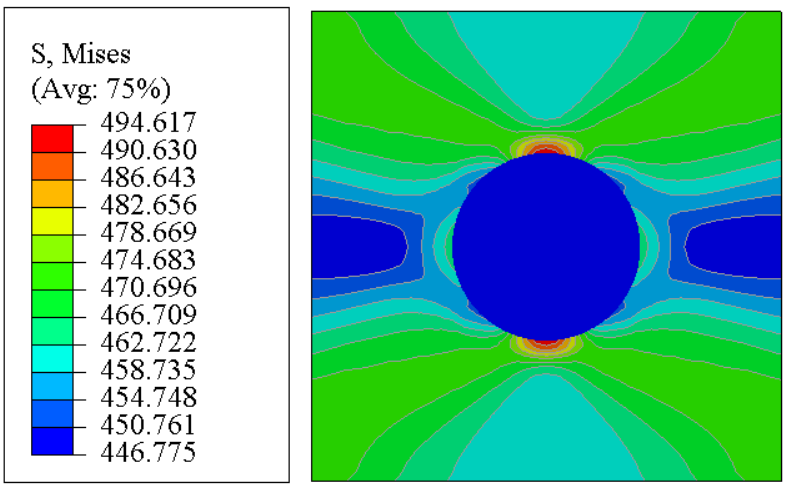
\includegraphics[width=\textwidth]{images/MISES_Coarse.png}
        \caption*{(a) $\sigma_{vM}$ for coarse mesh}
    \end{minipage}
    \hfill
    \begin{minipage}{0.48\textwidth}
        \centering
        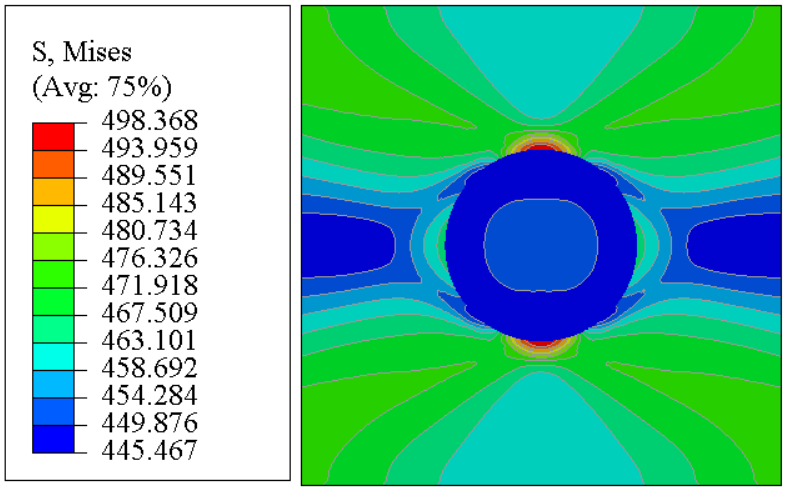
\includegraphics[width=\textwidth]{images/MISES_Fine.png}
        \caption*{(b) $\sigma_{vM}$ for fine mesh}
    \end{minipage}
    \vspace{1em}
    \begin{minipage}{0.48\textwidth}
        \centering
        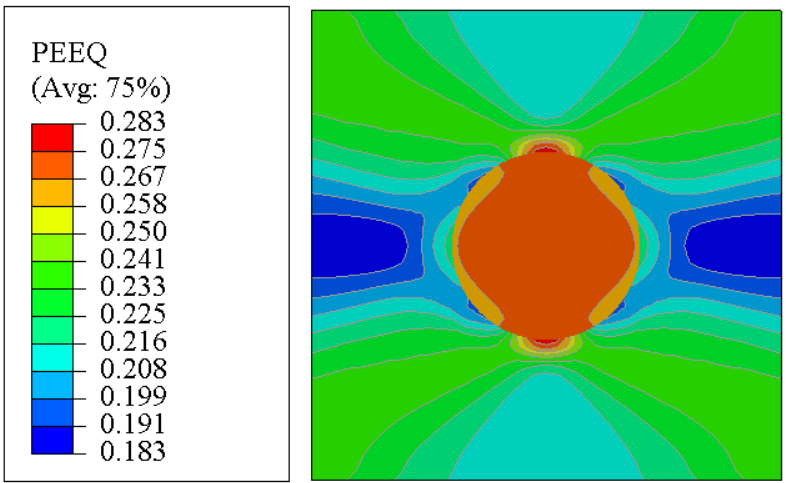
\includegraphics[width=\textwidth]{images/PEEQ_Coarse.png}
        \caption*{(c) $\varepsilon_{vM}$ for coarse mesh}
    \end{minipage}
    \hfill
    \begin{minipage}{0.48\textwidth}
        \centering
        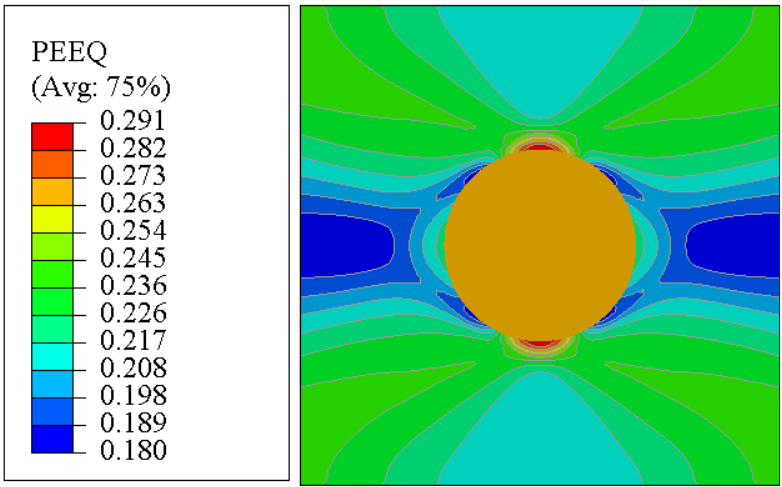
\includegraphics[width=\textwidth]{images/PEEQ_Fine.png}
        \caption*{(d) $\varepsilon_{vM}$ for fine mesh}
    \end{minipage}
    \caption{Comparison of von Mises stress $\sigma_{vM}$ and equivalent plastic strain $\varepsilon_{vM}$ distribution 
    for coarse (a, c) and fine (b, d) mesh 
    sizes for 1536 and 6144 nodes, respectively. Noted that all the used unit for von Mises stress plot is MPa for stress unit 
    and mm/mm for strain unit.}
    \label{fig:stressFields}
\end{figure}

\newpage
\subsection*{Q5: Comparison Analysis at Point B}
\textit{$\dots$Calculate Hill’s equivalent stress and equivalent plastic strain at point B in Figure 2 based on
the analytical equations given in the lecture and the components from the simulation.}
\vspace{1em}

Using equation~\ref{eq:hill_yield} and~\ref{eq:equivalent_plastic_strain}, we can calculate the Hill's equivalent stress and 
equivalent plastic strain at point B analytically. First, we need to extract the stress and strain
components from Abaqus using the same method as in the previous question 4. Following are the extracted value
at point B:

\begin{table}[H]
    \centering
    \caption{Extracted stress and strain components at point B from Abaqus.}
    \label{tab:pointA-results}
    \begin{tabular}{llllll}
        \toprule
        $\sigma_{11}$ (MPa) & $\sigma_{22}$ (MPa) & $\sigma_{12}$ (MPa) & $\varepsilon_{pl,11}$ & $\varepsilon_{pl,22}$ & $\varepsilon_{pl,12}$\\
        \midrule
        15.74 & 458.18 & 0 & -0.1629 & 0.2555 & 0\\
        \bottomrule
    \end{tabular}
\end{table}

For F, G, and H, we can use the values from the material B properties
\begin{align*}
F &= \frac{1}{2} \left[ \frac{1}{(R_{22})^2} + \frac{1}{(R_{33})^2} - \frac{1}{(R_{11})^2} \right] = \frac{1}{2} \left[ \frac{1}{(1.2)^2} + \frac{1}{(1.25)^2} - \frac{1}{(1)^2} \right] = 0.1672\\
G &= \frac{1}{2} \left[ \frac{1}{(R_{33})^2} + \frac{1}{(R_{11})^2} - \frac{1}{(R_{22})^2} \right] = \frac{1}{2} \left[ \frac{1}{(1.25)^2} + \frac{1}{(1)^2} - \frac{1}{(1.2)^2} \right] = 0.4728\\
H &= \frac{1}{2} \left[ \frac{1}{(R_{11})^2} + \frac{1}{(R_{22})^2} - \frac{1}{(R_{33})^2} \right] = \frac{1}{2} \left[ \frac{1}{(1)^2} + \frac{1}{(1.2)^2} - \frac{1}{(1.25)^2} \right] = 0.5277
\end{align*}    

Therefore, we can calculate the Hill's equivalent stress at point B as follows:
\begin{equation}
    \sigma_{eq, hill}^B = \sqrt{0.1672(458.18-0)^2 + 0.5277(0-15.74)^2 + 0.5277(15.74-458.18)^2}
\end{equation}

\begin{equation}
    \sigma_{eq, hill}^B = 372.11 \;\text{MPa}
\end{equation}

Finally, we can calculate the hill's equivalent plastic strain at point B as follows:
\begin{equation}
    \varepsilon_{eq}^B = \sqrt{\frac{0.1672(-0.1629)^2 +0.4728(0.2555)^2 + 0.5277(0.2555+(-0.1629))^2}{0.1672 \cdot 0.4728 + 0.5277 \cdot 0.4728 + 0.1672 \cdot 0.5277}}
\end{equation}
\begin{equation}
    \varepsilon_{eq}^B = 0.3091
\end{equation}

\newpage
\subsection*{Extra Task}
To calculate $\frac{\partial{f}}{\partial{\sigma}}$ with Voigt notation tensor $\sigma = (\sigma_1, \sigma_2, \sigma_3, \sigma_4, \sigma_5, \sigma_6)$ from yield function 
$f(\sigma)=\sigma_{eq} - \sigma_y$, where $\sigma_{eq}$ can be described as follows:

\begin{equation}
    \sigma_{eq} = \sqrt{\frac{1}{2} \left( H_{1}(\sigma_1 - \sigma_2)^2 + H_{2}(\sigma_2 - \sigma_3)^2 + H_{3}(\sigma_3 - \sigma_1)^2 + 6H_{4}\sigma_4^2 + 6H_{5}\sigma_5^2 + 6H_{6}\sigma_6^2 \right)}
\end{equation}

Hence, we can simplify the prescribed equation to:

\begin{equation}
A = \frac{1}{2} \left( (\sigma_1 - \sigma_2)^2 + (\sigma_2 - \sigma_3)^2 + (\sigma_3 - \sigma_1)^2 + 6(\sigma_4^2 + \sigma_5^2 + \sigma_6^2) \right)
\end{equation}

We can substitute the equation above into the yield function $f(\sigma)$ and applying the chain rule in the 
derivative, we obtain:

\begin{equation}
f(\sigma) = \sqrt{A} - \sigma_y \rightarrow \frac{\partial{f}}{\partial{\sigma}} = \frac{\partial{f}}{\partial{A}} \cdot \frac{\partial{A}}{\partial{\sigma}} = \frac{1}{2\sqrt{A}} \cdot \frac{\partial{A}}{\partial{\sigma}}
\end{equation}

Since we defined $A$ as a substituent of the equivalent stress $\sigma_{eq}$, we can revert the equation as in the origin form:

\begin{equation}
    \frac{\partial{f}}{\partial{\sigma}} = \frac{1}{2\sigma_{eq}} \cdot \frac{\partial{A}}{\partial{\sigma}}
\end{equation}

Now we need to expand the tensor differential with respect to each stress component in 
the Voigt notation. Therefore, we can do the differential operation for each stress 
component and assemble them to a Voigt notation as following sequence:

\[
\frac{\partial{A}}{\partial{\sigma_1}} = H_{1}(\sigma_1-\sigma_2) + H_3(\sigma_1-\sigma_3) \;;
\]
\[
\frac{\partial{A}}{\partial{\sigma_2}} = H_{2}(\sigma_2-\sigma_3) + H_1(\sigma_2-\sigma_1) \;;
\]
\[
\frac{\partial{A}}{\partial{\sigma_3}} = H_{2}(\sigma_3-\sigma_2) + H_3(\sigma_3-\sigma_1) \;;
\]
\[
\frac{\partial{A}}{\partial{\sigma_4}} = 6H_{4}\sigma_4 \;;
\]
\[
\frac{\partial{A}}{\partial{\sigma_5}} = 6H_{5}\sigma_5 \;;
\]
\[
\frac{\partial{A}}{\partial{\sigma_6}} = 6H_{6}\sigma_6 \;;
\]

To summarize the above equations, we can write them in a matrix form as follows:
\begin{equation}
\frac{\partial{f}}{\partial{\sigma}} = \frac{1}{2\sigma_{eq}}\begin{bmatrix}
H_{1}(\sigma_1-\sigma_2) + H_3(\sigma_1-\sigma_3) \\    
H_{2}(\sigma_2-\sigma_3) + H_1(\sigma_2-\sigma_1) \\
H_{2}(\sigma_3-\sigma_2) + H_3(\sigma_3-\sigma_1) \\
6H_{4}\sigma_4 \\
6H_{5}\sigma_5 \\
6H_{6}\sigma_6
\end{bmatrix}
\end{equation}




\section*{Conclusion}
To sum up everything that have been analyzed and gathered in this study, 
here are some several key takeaways from this small case study:
\begin{enumerate}
    \item The mechanical response of the homogeneous plate and the plate with circular inclusion was analyzed 
    using both direct and calculated stress-strain methods, 
    highlighting the differences between engineering and true stress-strain curves.
    \item Plane stress and plane strain conditions were compared, 
    showing that plane strain produced slightly higher stresses due to deformation constraints in the thickness direction.
    \item The inclusion of a softer, anisotropic material led to a reduction in yield and fracture stresses, 
    but the overall elastic modulus remained dominated by the non-inclusion/
    matrix material.
    \item Local stress field analysis revealed stress concentrations at the inclusion boundary and differences 
    in stress components due to material discontinuity.
    \item Analytical calculations of equivalent stress and plastic strain at specific points 
    matched closely with simulation results, validating the numerical approach.
    \item Mesh refinement had a minor effect on the results, indicating mesh independence for the chosen mesh sizes.
    \item The analytical derivation of the yield function gradient in Voigt notation was demonstrated for further 
    theoretical understanding.
\end{enumerate}

\end{document}

